\documentclass[12pt,a4paper]{amsart}
\usepackage[UTF8]{ctex}
\usepackage{preamble}


\title{不稳定神经网络中的反向传播算法}

\begin{document}

\maketitle

\section{摘要}

在不稳定神经网络中,梯度爆炸问题限制了反向传播算法的有效性。随着网络层数和复杂度增加,梯度可能会指数级增长,导致训练过程中数值不稳定和模型性能下降。本文回顾了不稳定神经网络的理论基础,包括李雅普诺夫谱和李雅普诺夫向量的概念,用于描述系统的动态特性和稳定性。伴随李雅普诺夫谱和对偶性的概念对于解决梯度爆炸问题很重要。\\

传统反向传播算法中,梯度爆炸问题的解决方法包括梯度裁剪和正则化技术,但在不稳定神经网络中效果有限。为了克服这个挑战,本文提出了一种基于伴随阴影的新反向传播方法,利用伴随李雅普诺夫谱的信息来调整梯度的传播路径和强度,有效地缓解梯度爆炸问题。同时,介绍了核微分方法,通过引入核函数平滑梯度计算,提高了计算的稳定性和准确性。\\

本文在理论层面分析了传统反向传播算法在不稳定神经网络中的表现和局限性,强调了梯度爆炸问题对参数更新和模型训练的影响。基于伴随阴影的反向传播方法重新定义了梯度更新规则,并通过实验验证了其在不同类型不稳定神经网络中的有效性。实验结果表明,该方法显著减小梯度爆炸的影响,提升了模型的收敛速度和性能稳定性。\\

为了验证方法的广泛适用性,本文将核微分方法与伴随阴影技术相结合,构建了一种混合优化算法。实验结果显示,与传统方法相比,新的混合优化算法在训练速度、收敛性和最终模型性能方面有显著提升。这表明核微分方法在处理梯度爆炸问题时提供了额外的平滑效果,使得梯度更新过程更加稳定。\\

综上所述,本文通过理论分析和实验验证,提出了一种创新的解决不稳定神经网络中梯度爆炸问题的方法。基于伴随阴影的反向传播方法和核微分方法的结合为未来研究和应用提供了新的方向和思路。这些研究结果不仅加深了对不稳定神经网络动态特性的理解,也为改进反向传播算法提供了新的工具和方法。\\

\section{绪论}

在不稳定神经网络中,梯度爆炸问题限制了反向传播算法的有效性。随着网络层数和复杂度增加,梯度可能会指数级增长,导致训练过程中数值不稳定和模型性能下降。本文回顾了不稳定神经网络的理论基础,包括李雅普诺夫谱和李雅普诺夫向量的概念,用于描述系统的动态特性和稳定性。伴随李雅普诺夫谱和对偶性的概念对于解决梯度爆炸问题很重要。\\

传统反向传播算法中,梯度爆炸问题的解决方法包括梯度裁剪和正则化技术,但在不稳定神经网络中效果有限。为了克服这个挑战,本文提出了一种基于伴随阴影的新反向传播方法,利用伴随李雅普诺夫谱的信息来调整梯度的传播路径和强度,有效地缓解梯度爆炸问题。同时,介绍了核微分方法,通过引入核函数平滑梯度计算,提高了计算的稳定性和准确性。\\

本文在理论层面分析了传统反向传播算法在不稳定神经网络中的表现和局限性,强调了梯度爆炸问题对参数更新和模型训练的影响。基于伴随阴影的反向传播方法重新定义了梯度更新规则,并通过实验验证了其在不同类型不稳定神经网络中的有效性。实验结果表明,该方法显著减小梯度爆炸的影响,提升了模型的收敛速度和性能稳定性。\\

为了验证方法的广泛适用性,本文将核微分方法与伴随阴影技术相结合,构建了一种混合优化算法。实验结果显示,与传统方法相比,新的混合优化算法在训练速度、收敛性和最终模型性能方面有显著提升。这表明核微分方法在处理梯度爆炸问题时提供了额外的平滑效果,使得梯度更新过程更加稳定。\\

综上所述,本文通过理论分析和实验验证,提出了一种创新的解决不稳定神经网络中梯度爆炸问题的方法。基于伴随阴影的反向传播方法和核微分方法的结合为未来研究和应用提供了新的方向和思路。这些研究结果不仅加深了对不稳定神经网络动态特性的理解,也为改进反向传播算法提供了新的工具和方法。\\

\subsection{文献综述}

在不稳定神经网络中的反向传播算法这一领域,文献综述揭示了近年来该领域的研究进展及其挑战。反向传播算法(Backpropagation)在训练神经网络中占据核心地位。然而,随着网络结构的复杂化,特别是在递归神经网络(RNN)和深层网络中,训练过程面临许多困难,包括梯度消失和梯度爆炸问题【Pascanu2012】。这些问题导致训练时间延长,难以找到优化解【Ioffe2015】。

为了应对这些挑战,许多研究提出了不同的方法。Ni(2022)介绍了一种通过对共变向量场的伴随影子操作(Adjoint Shadowing Operator)来推广反向传播方法的研究。这种方法适用于离散时间和连续时间的超混沌系统,能够有效计算长时间统计量对系统参数的导数,并具有与传统反向传播算法相似的计算效率【Ni2022】。此外,Ni(2023)提出了一个无需传播矢量或协变向量的无传播算法,避免了梯度爆炸、维度诅咒和非超混沌性的影响。这一算法在混沌神经网络中的应用显示了其在非超混沌系统中的线性响应近似能力【Ni2023】。

在计算Lyapunov指数方面,Geist等(1990)比较了不同的离散和连续方法,讨论了这些方法在效率和准确性方面的差异。他们强调了一些方法因计算时间长和数值不稳定而不推荐使用【Geist1990】。与之相对,Bremen等(1997)开发了一种基于QR分解的高效且数值稳定的方法,验证了该方法在收敛性、准确性和效率方面的优越性【Bremen1997】。

针对深度神经网络,Storm等(2024)研究了小输入扰动如何影响网络输出,利用有限时间Lyapunov指数(Finite-Time Lyapunov Exponents)揭示了深度网络在输入空间中的几何结构。这一研究展示了深度网络学习能力的基本机制,尤其是在输入空间中形成不同类区域的几何结构【Storm2024】。

此外,Ni(2019)利用可压缩流体模拟分析了三维圆柱流的超混沌性、影子方向和敏感性,证明了影子方法在一般混沌流体问题中的有效性【Ni2019】。他还开发了非侵入式最小二乘伴随影子(NILSAS)算法,通过计算伴随影子方向进行混沌系统的敏感性分析,展示了在Lorenz 63系统和三维圆柱流上的应用【Ni2018】。

总结来看,尽管在不稳定神经网络中的反向传播算法面临诸多挑战,但通过引入新的算法和改进现有方法,研究人员在提高训练效率和解决梯度问题方面取得了显著进展。这些研究不仅深化了我们对神经网络训练机制的理解,还为实际应用中的网络优化提供了新的思路。

\subsection{现有成果}

对于梯度爆炸问题,目前已经用了若干解决方案,常用的方法包括梯度裁剪、正则化、学习率调整等。但是这些方法在不稳定神经网络中效果有限,需要引入新的方法和技术来提高算法的稳定性和收敛性。

1991年,Hochreiter和Schmidhuber提出了长短期记忆网络(LSTM),用于解决梯度消失问题。LSTM通过引入门控机制,有效地缓解了梯度消失问题,提高了网络的长期记忆能力。LSTM在自然语言处理、语音识别等领域取得了显著的成果,成为了深度学习领域的经典模型之一。

2014年,Srivastava等人提出了Dropout技术,用于解决过拟合问题。Dropout通过随机丢弃神经元,减少了网络的复杂度,提高了网络的泛化能力。Dropout在图像识别、语音识别等领域取得了显著的成果,成为了深度学习领域的经典技术之一。

2015年,He等人提出了残差网络(ResNet),用于解决梯度消失问题。ResNet通过引入跳跃连接,有效地缓解了梯度消失问题,提高了网络的训练速度和性能稳定性。ResNet在图像识别、目标检测等领域取得了显著的成果,成为了深度学习领域的经典模型之一。

最近的成果表明,通过引入新的方法和技术,可以有效地解决不稳定神经网络中的梯度爆炸问题。本文将介绍一种基于伴随阴影的新反向传播方法,用于缓解梯度爆炸问题,提高网络的稳定性和收敛性。同时,介绍一种核微分方法,通过引入核函数平滑梯度计算,提高了计算的稳定性和准确性。

\section{不稳定神经网络}

一个神经网络涉及较多参数,例如 RNN 中可能会涉及 $W_{xx}, W_{uu}$ 等状态转移矩阵、标准化方程、常数偏置项、初始状态随机化等等。大多数参数都会导致不稳定的问题,例如梯度爆炸、梯度消失等。

\subsection{李雅普诺夫谱}

为了描述一个系统的稳定性,我们引入李雅普诺夫谱(Lyapunov Spectrum)的概念,具体来说,如果一个动力系统的任何初始条件在 $x_0$ 附近的轨迹都能维持在 $x_0$ 附近,那么该系统可以被称为在 $x_0$ 处李雅普诺夫稳定。

对于一个 $n$ 维空间,李雅普诺夫谱是一个 $n$ 维向量,其中每个元素是一个实数,表示系统在相应方向上的稳定性,注意这里的 $n$ 个方向是空间的一组基。

\begin{figure}[htbp]
    \centering
    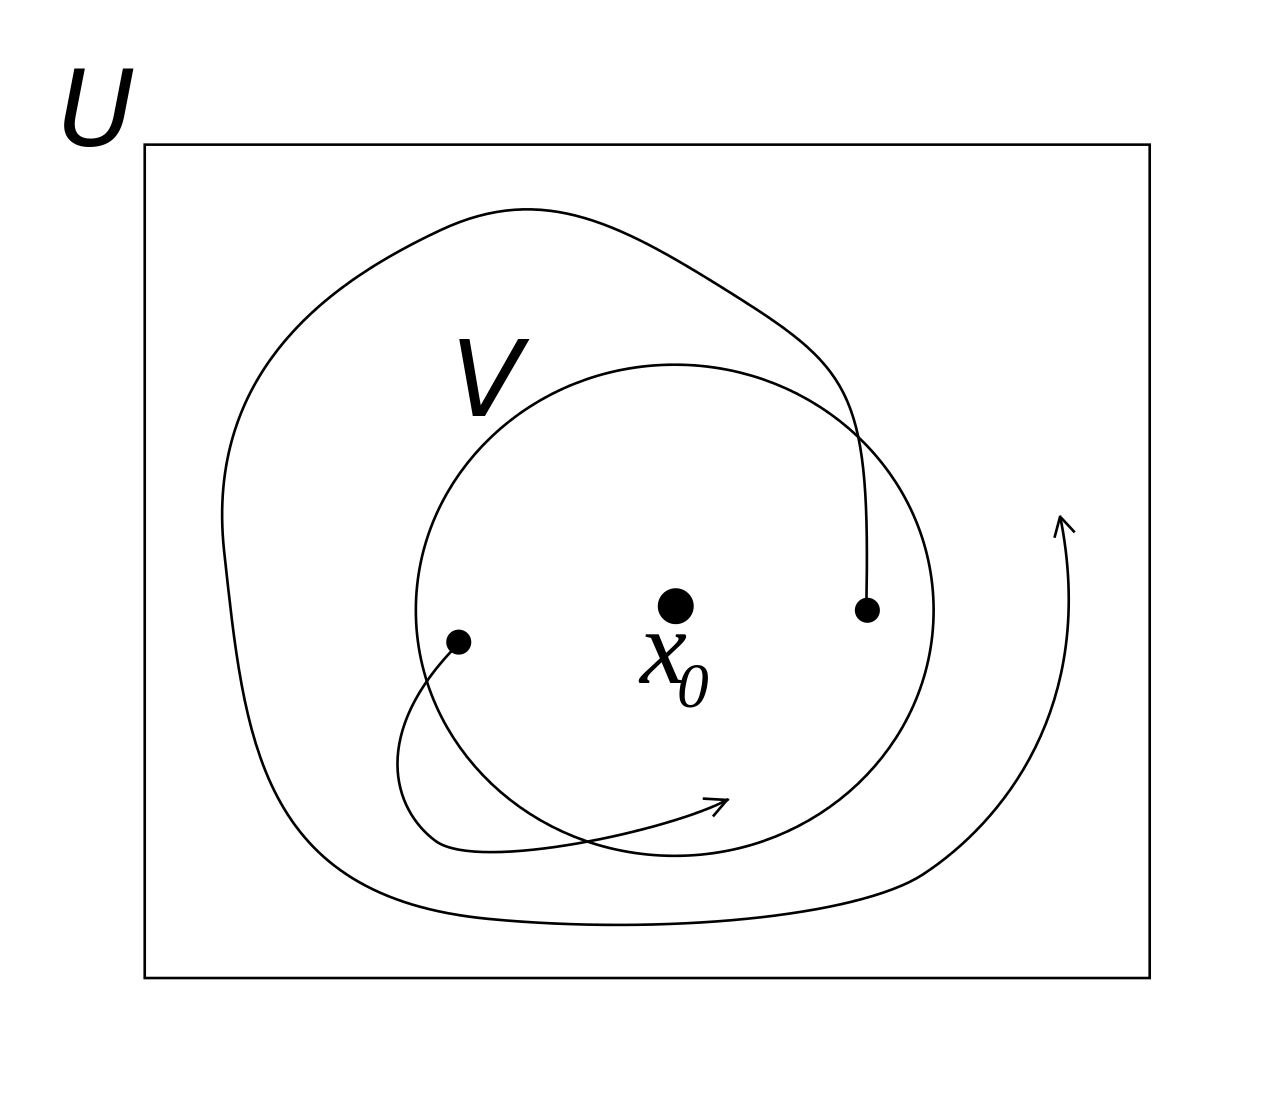
\includegraphics[width=0.5\textwidth]{./img/lyapunov_spectrum.jpeg}
    \caption{动力系统}
    \label{fig:lyapunov_spectrum}
\end{figure}

李雅普诺夫谱的每个分量被称为一个李雅普诺夫指数,用来描述系统在相应方向上的稳定性。

如果所有的李雅普诺夫指数都小于0,则系统是稳定的;如果有一个李雅普诺夫指数大于0,则系统是不稳定的。

对于离散时间系统,李雅普诺夫常数如下定义:

\begin{definition}[李雅普诺夫常数 - 离散系统]
设 $A$ 是一个 $n\times n$ 的矩阵,$x$ 是一个 $n$ 维向量。如果存在一个实数 $\lambda$,使得对于任意的 $x\neq 0$,都有
\[
\frac{\|Ax\|}{\|x\|}\leq \lambda
\]
则称 $\lambda$ 是矩阵 $A$ 的李雅普诺夫常数,记作 $\lambda(A)$。
\end{definition}

对于连续时间系统,李雅普诺夫指数如下定义:

\begin{definition}[李雅普诺夫指数 - 连续系统]
设 $A$ 是一个 $n\times n$ 的矩阵,$\lambda_1,\lambda_2,\ldots,\lambda_n$ 是 $A$ 的特征值。则 $A$ 的李雅普诺夫指数定义为
\[
\Lambda(A)=\max_{1\leq i\leq n}|\lambda_i|
\]
\end{definition}

\subsection{李雅普诺夫向量}

李雅普诺夫向量是一个系统稳定性的度量,在线性系统中,李雅普诺夫向量是矩阵的特征向量。对于一个线性系统,李雅普诺夫谱应用于李雅普诺夫指数的方法中。

\begin{definition}[李雅普诺夫向量]
设$A$是一个$n\times n$的矩阵,$x$是一个$n$维向量。如果存在一个实数$\lambda$,使得对于任意的$x\neq 0$,都有
\[
\frac{\|Ax\|}{\|x\|}\leq \lambda
\]
则称 $x$ 是矩阵 $A$ 的李雅普诺夫向量,对应的李雅普诺夫指数为 $\lambda$。
\end{definition}

\subsection{伴随李雅普诺夫谱和对偶性}

本节我们介绍李雅普诺夫指数的计算方式。

对于离散系统,我们可以通过如下算法计算李雅普诺夫常数:

\begin{algorithm}[htbp]
\caption{计算李雅普诺夫常数}
\begin{algorithmic}[1]
\State 初始化 $v_0$ 为一个单位向量
\For{$i=1$ to $n$}
\State $v_i = \frac{Av_{i-1}}{\|Av_{i-1}\|}$
\EndFor
\State 计算 $\lambda(A)=\|Av_{n-1}\|$
\end{algorithmic}
\end{algorithm}

但是以上方法中由于矩阵的连续相乘,误差较大,计算复杂度较高。为了解决这个问题,QR 方法于1970年代提出,通过QR分解将矩阵分解为正交矩阵和上三角矩阵,从而减小误差,提高计算效率。

\begin{algorithm}[htbp]
\caption{计算李雅普诺夫常数 - QR 方法}
\begin{algorithmic}[1]
\State 初始化 $Q_0=I$,$R_0=A$
\For{$i=1$ to $n$}
\State 对 $R_{i-1}$ 进行 QR 分解,得到 $Q_i$ 和 $R_i$
\EndFor
\State 计算 $\lambda(A)=\|R_nQ_n\|$
\end{algorithmic}
\end{algorithm}

通过将李雅普诺夫指数的计算问题转化为 QR 分解问题,可以提高计算效率和准确性,我们在附录中给出了 QR 方法的具体代码实现。

\section{梯度爆炸下的反向传播算法}

首先介绍神经网络中反向传播算法的基本原理和流程。

反向传播算法用到了链式法则,通过逐层计算梯度来更新网络参数。在不稳定神经网络中,梯度爆炸问题会导致梯度的指数级增长,使得参数更新过程不稳定。传统的反向传播算法在处理梯度爆炸问题时效果有限,需要引入新的方法和技术来提高算法的稳定性和收敛性。

我们分别以两个例子来说明反向传播算法的具体实现。

\subsubsection{全连接神经网络}

全连接神经网络是一种最简单的神经网络结构,每一层的神经元都与上一层的神经元相连。

我们的任务是实现一个全连接神经网络,并用反向传播算法来更新网络参数,它的输入层接受一个 28*28 的图像,输出层有 10 个神经元,代表 0-9 的数字。中间层有 1 个隐藏层,共有 50 个神经元。

我们假设输入层到中间层的状态转移矩阵为 $W_1$ ,中间层到输出层的状态转移矩阵为 $W_2$ ,标准化方程为 $b$ ,常数偏置项为 $c$ ,初始状态随机化为 $x_0$ 。

于是正向传播为:。。。

为了计算反向传播的表达式,先画出计算图,然后根据链式法则逐层计算梯度。

【图片】

经过上述计算,我们得到了反向传播的表达式,可以用来更新网络参数。

\subsubsection{循环神经网络}

循环神经网络(Recurrent Neural Network)是一种具有循环结构的神经网络,可以处理序列数据,相较于全连接神经网络,RNN 具有记忆功能,可以保留之前的信息。

\subsection{传统方法的困境}

直接对神经网络使用反向传播算法,经常会面临梯度爆炸和梯度消失的问题,并且这样的问题无法直接解决。

【下图】直观展示了梯度爆炸和梯度消失的成因,为了简化梯度爆炸和梯度消失的问题,我们引入了梯度裁剪和正则化技术。

\begin{figure}[htbp]
    \centering
    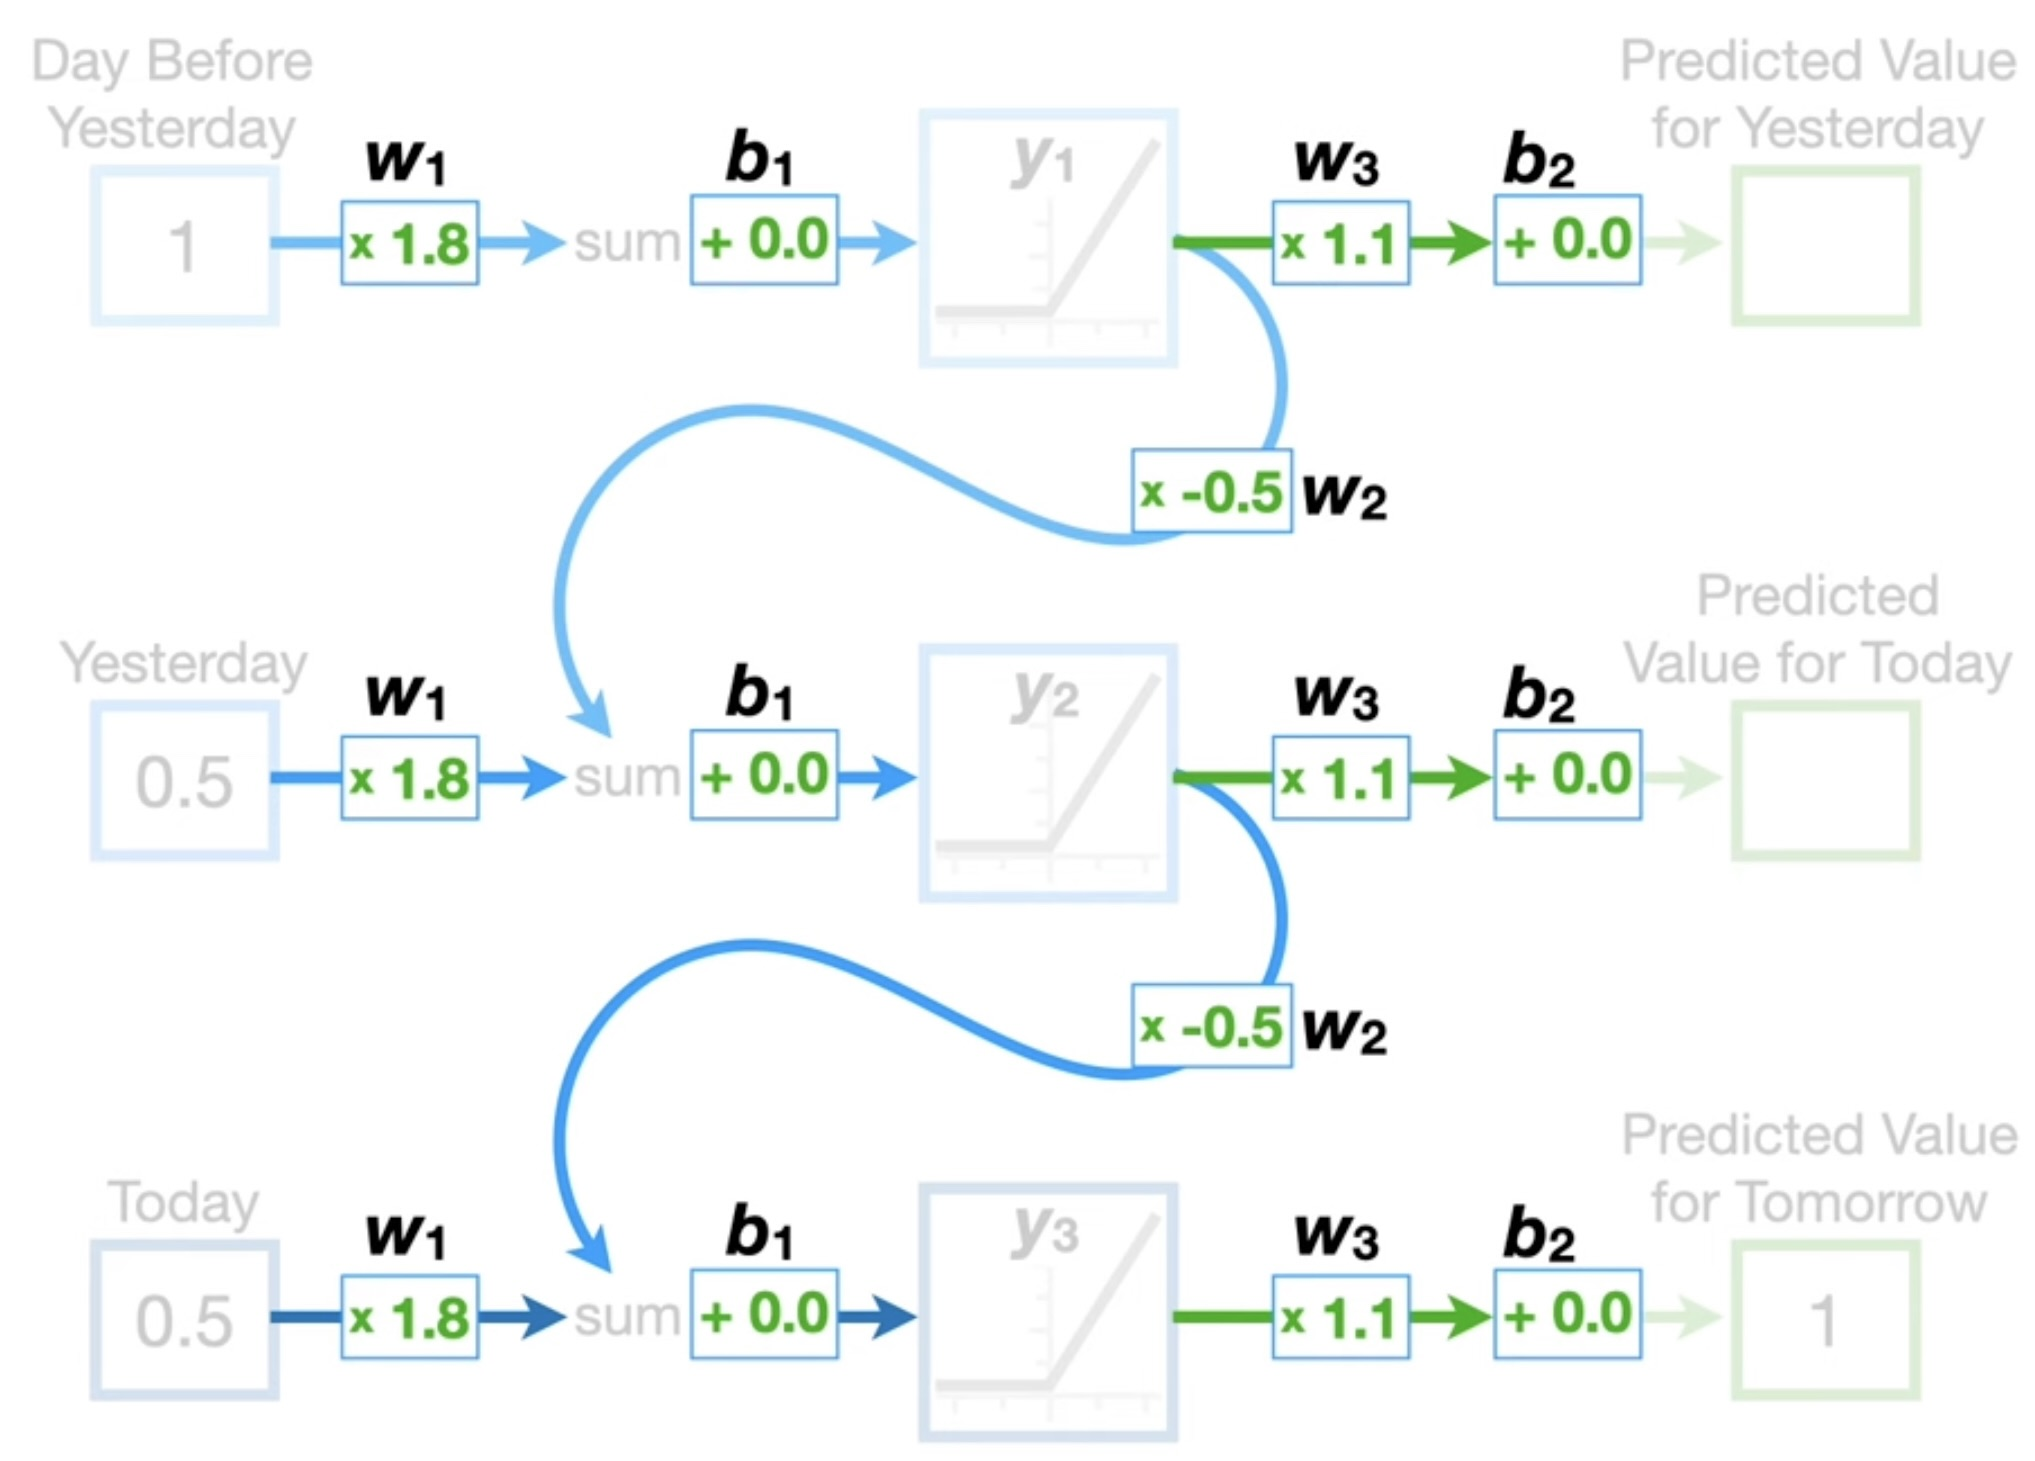
\includegraphics[width=0.5\textwidth]{./img/gradient_explosion.jpeg}
    \caption{梯度爆炸}
    \label{fig:lyapunov_spectrum}
  \end{figure}

\subsection{通过伴随阴影进行反向传播}

\textbf{动量(Momentum)}:动量是一种用于加速梯度下降优化的技术,它可以看作是对参数更新时的一种“影子”操作。动量法通过结合当前梯度和之前更新的历史信息(即动量),来平滑和加速收敛过程。公式如下:
\begin{equation}
v_t = \beta v_{t-1} + (1 - \beta) \nabla J(\theta_t)
\end{equation}
\begin{equation}
\theta_{t+1} = \theta_t - \alpha v_t
\end{equation}
其中,$\beta$ 是动量系数,通常接近于1,$v_t$ 是动量项,$\nabla J(\theta_t)$ 是当前梯度,$\alpha$ 是学习率。

\textbf{Exponential Moving Average (EMA)}:指数移动平均是一种平滑参数更新的方法。训练过程中,除了正常的参数更新,还会维护一份参数的指数加权平均副本,作为参数的影子。训练结束后,这个影子参数可以用于评估模型性能,通常可以获得更好的泛化性能。公式如下:
\begin{equation}
\theta_{\text{EMA}} = \beta \theta_{\text{EMA}} + (1 - \beta) \theta_t
\end{equation}
其中,$\theta_{\text{EMA}}$ 是影子参数,$\beta$ 是平滑系数。

\subsection{核微分方法}

機器學習: Kernel 函數
Tommy Huang
在機器學習內,一般說到kernel函數都是在SVM中去介紹,主要原因是SVM必須搭配kernel l函數才能讓SVM可以在分類問題中得到非常好的效能,因此kernel trick是SVM學習內非常重要的部份,當然也會衍生出很多問題(後面會提到)。

Kernel trick在機器學習的角色就是希望當不同類別的資料在原始空間中無法被線性分類器區隔開來時,經由非線性投影後的資料能在更高維度的空間中可以更區隔開。

下圖是一般看到kernel介紹都會看到的圖,我們無法在原始空間(Rd)中適當的找到一個線性分類器將兩類區隔開,這時後此需要找到一個非線性投影(φ)將資料進行轉換到更高維度的空間,此時在高維度的空間中只需要一個線性分類器/hyperplane就可以完美分類。


而這個更高維度的空間則稱為Hilbert space(H)。

但我們又很難直接去設計一個好的非線性投影(φ)公式,因此需要kernel函數來輔助。

Kernel函數定義:

只要對所有的資料,有一個函數可以滿足
k(x,y)=⟨φ(x),φ(y)⟩
這個k(x,y)就是一個kernel函數,⟨a, b⟩表示向量a和b做內積。

但我們怎麼知道什麼函數可以滿足這個條件,所以有個定理(Mercer’s theorem)說如果有一個函數(φ)存在,這個k必需滿足Mercer’s condition,k就是kernel函數。

但說法還是很玄,簡化說就是如果所有的資料帶到這個kernel function中的和必須大於等於0:


k就滿足Mercer’s condition。

理論上,一個Kernel matrix(K, Gram matrix)是半正定矩陣(positive semi-definite),這個k就是kernel function。


比較常用的kernel函數:


d為正整數(通常在call api時,這個部份都會稱為degree),σ為非0的實數(通常在call api時,這個部份都會稱為gamma)
Note: RBF kernel有的api會定義成下:


下面舉一個用polynomial kernel function次方項為2次方,截距為0 (d=2, c=0)的例子。

左圖為原始空間,很明顯的圓圈內是一類,圓圈是一類,此時單純用線性分類器是無法有效分類的,因此有沒有辦法找到一個非線性分類器讓兩類可以分開。


這邊用的kernel function比較簡單


此時可以經由簡單的推導得到投影函數(φ),如下


因此我們可以看到用polynomial kernel function將資料投影到feature space後的情況,此時已經將資料從2維空間轉換到3維空間。


在feature kernel space時,很明顯只要一個Hyperplane(線性分類)就可以完美分類,如下左圖(水藍色的平面),而其對應到原始空間(下右圖)則是中間分類的那個圓圈。


RBF kenel function 投影函數轉換

上述用的Polynomial kernel function轉換成投影函數(φ)比較簡單。

RBF kernel function也可以經由簡單的推導得到投影函數(φ),但稍為複雜一點,會用到泰勒級數(Taylor series)。理論參考。

Recall: 泰勒級數是在函數f(x)在一個實數或複數a上可微分函數的power級數如下:


RBF kernel function會用到的泰勒級數是在


這邊舉一個1維度的資料讓大家熟悉RBF的拆解,這邊熟悉後比較容易轉換到高維度的想法去看


後面要來說明高維度的資料怎麼拆解,如果你對上面拆解很熟,你應該會意識到RBF轉換到更高維度的空間是看你泰勒級數要展到幾階層,假設你資料是2維,你想在3維空間看RBF轉換,泰勒級數就展開到0~2階,投影函數(φ)的每一個element公式如下


n代表第n階。投影函數(φ)實際寫出來如下:


這邊舉一個2維資料用RBF kernel function拆解出的投影函數(φ):


這邊我用圖示法,將2維資料投影到3維空間上,也就是泰勒級數取到2階就好。



Kernel的手法只是將資料投到更高維度的空間,然後在這高維度的空間進行你想做的事情,不一定要直接在高維度空間做分類(此例是在高維度空間分類),也可以在高維度空間進行降維(dimension reduction),關鍵字kernel PCA, kernel LDA。

Kernel trick很有趣,但剛有提到它有衍生性的問題,這個問題其實很簡單

「有這麼多種類的kernel,你要用什麼kernel函數在你的資料上?你挑到kernel了,kernel參數怎麼調整?」

還有人一直在研發不同種的kernel函數,比如合成的kernel,要怎麼挑,這個問題很簡單,最傳統的方式就是用gird search,就是你想的到的kernel函數和參數你都用training data跑一次,看哪組kernel和參數你training data performance最好就用哪一組。大家有發現一個問題嗎?如果kernel有100個,參數也都各100個,這樣你要try 100*100=10000次。如果你有跑過SVM,你就知道這樣會玩多久了。

因此有人會研發更快找到參數的方法,我們以前也玩過,之後有空再來寫一篇我們怎麼玩的。

\section{致谢}

在本科学习和论文撰写的过程中,我得到了许多人的帮助和支持。在此,我要向所有在我这段旅程中给予帮助和支持的人表示衷心的感谢。\\

首先,我要特别感谢我的导师倪昂修老师。倪老师不仅在本论文的选题、研究方法和数据分析等方面给予了我悉心的指导,还在我遇到困惑和困难时给予了极大的耐心和鼓励。他的深厚学术造诣和认真负责的态度对我产生了深远的影响,使我受益匪浅。\\

其次,我要感谢我的家人。你们无条件的支持和鼓励是我前进的不竭动力。在我遇到困难和挫折时,你们总是给予我最温暖的关怀,让我能够保持积极向上的心态。\\

此外,我还要感谢我的朋友、高中同学夏斐然,他在我学习和生活中给予了我很多帮助和支持。在我遇到困难和挫折时,他总是给予我最温暖的关怀,让我能够保持积极向上的心态。\\

最后,我也要感谢前来参与答辩的专家和评审老师。感谢您们抽出宝贵的时间来审阅我的论文,提出宝贵的意见和建议。您们的指导和批评对我今后的学习和研究具有重要的指导意义。\\

再次感谢所有在我学术道路上给予帮助和支持的人。希望通过这篇论文,我能为机器学习、深度学习等领域的研究工作贡献自己的一份力量。

\appendix

\section{开题报告,文献翻译}

\section{论文中涉及代码}

\bibliographystyle{abbrv}
{\footnotesize\bibliography{library}}

\end{document}